\documentclass[12pt]{article}
\usepackage[charter, cal=cmcal]{mathdesign}
\usepackage[margin=1in]{geometry}
\usepackage[T1]{fontenc}
\usepackage{amsmath}
\usepackage{graphicx}
\usepackage{booktabs}
\usepackage{threeparttable}
\usepackage{natbib}
\usepackage{setspace}
\usepackage{hyperref}
\hypersetup{
    colorlinks=true,
    linkcolor=blue,
    citecolor=black,
    urlcolor=blue
}
\usepackage{placeins}

\onehalfspacing
\newcommand{\DelhiWomen}{68}
\newcommand{\DelhiPedestrians}{318}
\newcommand{\DelhiShare}{21.4}
\newcommand{\DelhiLo}{14.6}
\newcommand{\DelhiHi}{28.2}
\newcommand{\MaxCityPedCount}{26}
\newcommand{\IncomeSlope}{\ensuremath{+3.6}}
\newcommand{\WithinRegionIncomeSlope}{\ensuremath{-0.3}}
\newcommand{\TotalRegions}{6}
\newcommand{\DrawnImages}{20,048}
\newcommand{\DownloadedImages}{19,646}
\newcommand{\EligibleCities}{543}
\newcommand{\CorpusCities}{688}
\newcommand{\TotalStrata}{12}
\newcommand{\WomenPedestrians}{6,698}
\newcommand{\UnclearShare}{71.8}
\newcommand{\MENAPedShare}{15.9}
\newcommand{\ECAPedShare}{49.4}
\newcommand{\TotalCities}{101}
\newcommand{\TotalCountries}{88}
\newcommand{\TotalImages}{19,531}
\newcommand{\TotalPedestrians}{18,633}
\newcommand{\TotalRiders}{3,599}
\newcommand{\TotalUnclear}{56,630}
\newcommand{\GlobalPedShare}{35.9}
\newcommand{\GlobalPedCILo}{32.4}
\newcommand{\GlobalPedCIHi}{39.5}
\newcommand{\GlobalAllShare}{32.2}
\newcommand{\GlobalTWShare}{12.7}
\newcommand{\MinCityPedShare}{0.0}
\newcommand{\MaxCityPedShare}{69.2}
\newcommand{\IndiaCities}{4}
\newcommand{\IndiaImages}{797}
\newcommand{\IndiaPedShare}{22.3}
\newcommand{\IndiaPedCILo}{18.8}
\newcommand{\IndiaPedCIHi}{25.8}
\newcommand{\SouthAsiaPedShare}{26.3}
\newcommand{\SouthAsiaPedCILo}{19.9}
\newcommand{\SouthAsiaPedCIHi}{32.7}


\title{Missing Women on Global Streets: A Research Note}
\author{Gaurav Sood}
\date{\today}

\begin{document}
\maketitle

\begin{abstract}
\noindent How absent are women from city streets around the world? Using \TotalImages{} person-filtered street-level photographs across \TotalCities{} cities in \TotalCountries{} countries from the Global Streetscapes corpus, we measure apparent gender composition among \TotalPedestrians{} classified pedestrians and \TotalRiders{} two-wheeler riders. Globally, women account for \GlobalPedShare\% (95\% CI: [\GlobalPedCILo\%, \GlobalPedCIHi\%]) of classified pedestrians and \GlobalTWShare\% of two-wheeler riders, ranging from \MinCityPedShare\% to \MaxCityPedShare\% across cities.
\end{abstract}

\section{Introduction}
Presence in public space is a direct, observable indicator of gender equity in freedom of movement, yet prior street-level audits have been limited to small purposive sites or single-country surveys \citep{viswanath2015safetipin, goel2022mobility, photoball2026}. Recent randomized street surveys in four Indian cities using wearable cameras \citep{karekurve2026streetscope} and Google Street View audits in three Indian cities \citep{sood2026streetsight} found that women make up roughly 20\% to 27\% of visible pedestrians. Whether that magnitude is distinctive to South Asia or varies systematically across regions and national income has remained unknown for lack of comparable, cross-national street-level measurement \citep{elrod2025sociability}.

\section{Data and Sampling Design}
We draw a reproducible stratified sample of 100 cities from the Global Streetscapes corpus \citep{hou2024globalstreetscapes} (688 cities; Mapillary and KartaView imagery). Eligibility requires at least 400 images and non-missing city population and World Bank GDP per capita PPP (543 eligible cities). Cities are stratified across 12 cells defined by 6 World Bank-derived regions (merging North America and Latin America \& Caribbean into Americas) crossed with within-region income halves. Regional quotas follow Bankier square-root allocation, and cities are drawn via Efraimidis--Spirakis $\sqrt{\text{population}}$ weighting with an unrepresented-country-first pass and a population-scaled per-country cap, yielding \TotalCities{} cities across \TotalCountries{} countries (with New Delhi included as a certainty benchmark).

Within each city, we filter on precomputed Mask2Former instance counts ($\text{Person} + \text{Rider} \ge 1$) to avoid empty-road frames and draw 100 images per city in Round 1 (\TotalImages{} images). Each full-resolution frame is coded using \texttt{muse-spark-1.3-contributor} for pedestrian women, pedestrian men, two-wheeler women, two-wheeler men, and unclear-sex detections.

\section{Results}
\begin{tabular}{@{}lrrrrrr@{}}
\toprule
Region & Cities & Images & Pedestrians & Women [95\% CI] & Women riders & Unclear \\
\midrule
Europe \& Central Asia & 26 & 7,478 & 7,609 & 49.4\% [46.2, 52.5] & 32.0\% & 74.5\% \\
East Asia \& Pacific & 18 & 4,872 & 3,645 & 42.8\% [37.7, 47.9] & 21.8\% & 76.5\% \\
Americas & 25 & 7,080 & 3,992 & 39.9\% [36.3, 43.5] & 11.7\% & 76.8\% \\
Sub-Saharan Africa & 12 & 3,582 & 3,722 & 29.7\% [26.6, 32.7] & 8.8\% & 74.4\% \\
South Asia & 9 & 2,589 & 4,877 & 26.4\% [20.4, 32.5] & 10.9\% & 61.5\% \\
MENA, Afg. \& Pak. & 11 & 3,193 & 3,549 & 16.0\% [9.7, 22.4] & 4.8\% & 62.2\% \\
All sampled cities & 101 & 28,794 & 27,394 & 36.0\% [32.5, 39.6] & 12.6\% & 71.9\% \\
\bottomrule
\end{tabular}


\begin{figure}[ht]
\centering
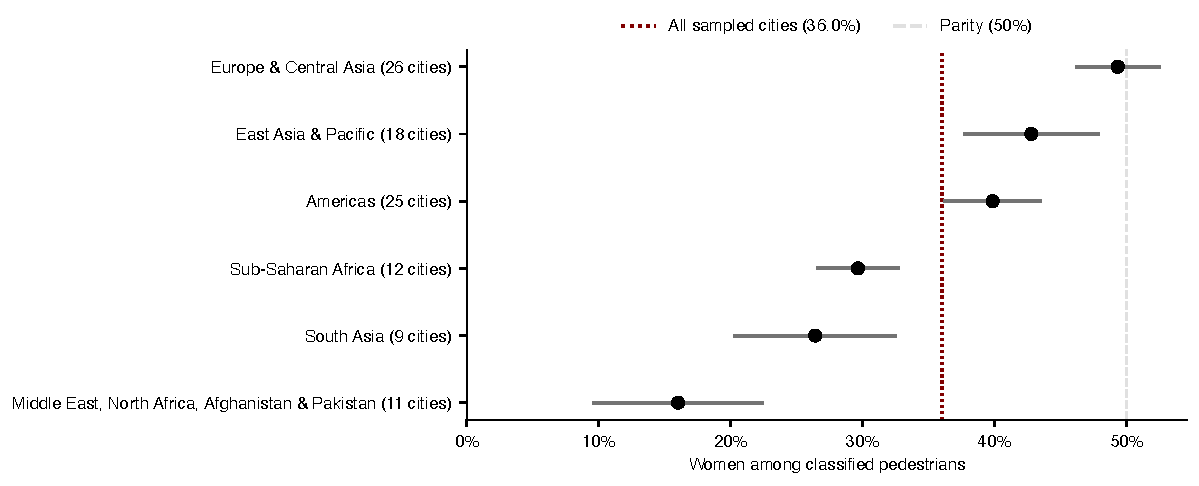
\includegraphics[width=0.92\textwidth]{../figs/fig1_region_summary.pdf}
\caption{Pedestrian female share across World Bank-derived regions with city-clustered 95\% confidence intervals. Dotted red line marks the global weighted mean (\GlobalPedShare\%); dashed gray line marks 50\% parity.}
\label{fig:region_summary}
\end{figure}

\begin{figure}[ht]
\centering
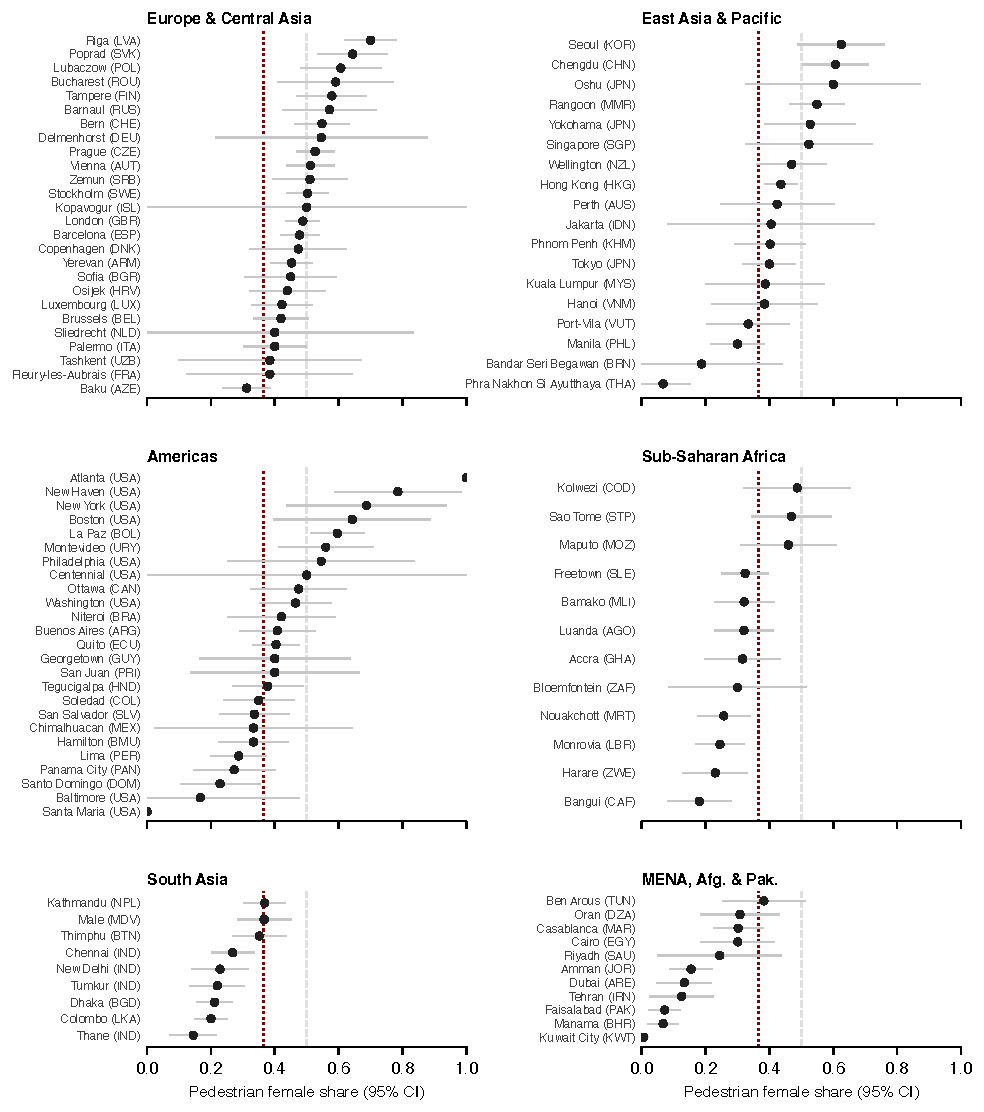
\includegraphics[width=0.92\textwidth]{../figs/fig2_city_distribution.pdf}
\caption{Distribution of pedestrian female share across \TotalCities{} sampled cities (95\% CIs clustered by image).}
\label{fig:city_dist}
\end{figure}

\begin{figure}[ht]
\centering
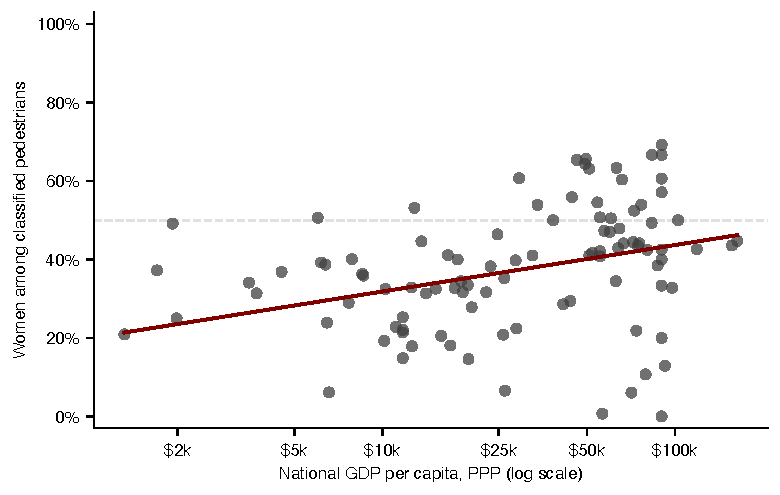
\includegraphics[width=0.88\textwidth]{../figs/fig3_gdp_vs_female_share.pdf}
\caption{National GDP per capita PPP (log scale) versus city-level pedestrian female share.}
\label{fig:gdp}
\end{figure}

\begin{figure}[ht]
\centering
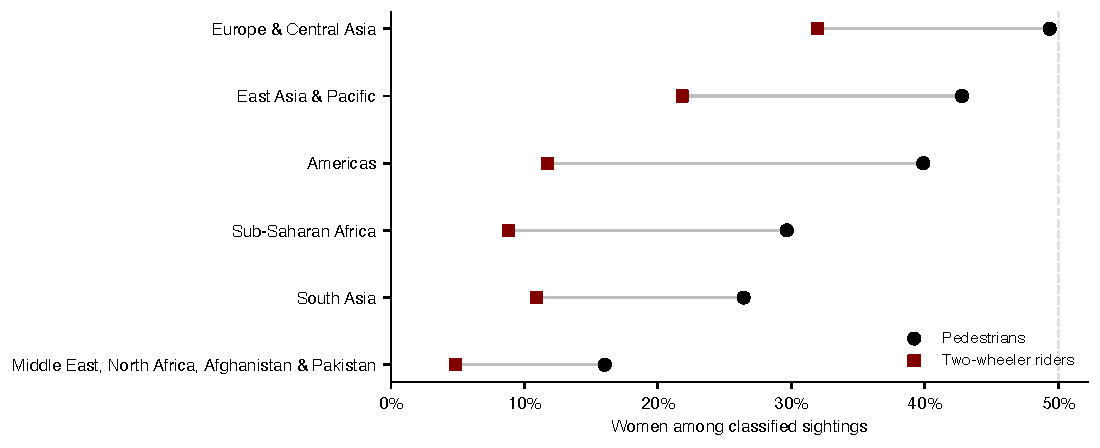
\includegraphics[width=0.88\textwidth]{../figs/fig4_pedestrian_vs_twowheeler.pdf}
\caption{Female share among pedestrians (circles) versus two-wheeler riders (squares) by region.}
\label{fig:modes}
\end{figure}

\FloatBarrier
\bibliographystyle{plainnat}
\bibliography{../docs/refs.bib}

\clearpage
\appendix
\section{Pixel-Area Threshold Sensitivity}
\begin{tabular}{@{}lrrrr@{}}
\toprule
Minimum pixels & Images kept & Pedestrians kept & Unclear & Women (ped.) \\
\midrule
0 & 19,531 (100.0\%) & 18,633 (100.0\%) & 56,630 & 35.95\% \\
1,000 & 16,929 (86.7\%) & 18,541 (99.5\%) & 53,907 & 36.01\% \\
2,000 & 15,184 (77.7\%) & 18,403 (98.8\%) & 50,980 & 36.07\% \\
5,000 & 11,615 (59.5\%) & 17,729 (95.1\%) & 43,609 & 36.16\% \\
10,000 & 8,719 (44.6\%) & 16,384 (87.9\%) & 36,003 & 36.62\% \\
20,000 & 6,110 (31.3\%) & 14,178 (76.1\%) & 27,299 & 37.16\% \\
\bottomrule
\end{tabular}


\end{document}
